\fontsize{13}{14}\selectfont
\chapter{Giới thiệu đề tài}
\newpage
\section{Product requirement}
\begin{enumerate}[label=\alph*)]
	\item \textbf{Name: } Thiết bị đo điện áp DC/AC và hiển thị dạng điện áp trên máy tính
	\item \textbf{Purpose: }
	\begin{itemize}[label=+]
		\item Đo các thông số giá trị của điện áp trong miền thời gian.
		\item Tiện lợi, dễ sử dụng, phục vụ cho các yêu cầu trong việc học tập nghiên cứu của học sinh, sinh viên.
	\end{itemize}
	\item \textbf{Inputs and outputs: }
	\begin{itemize}[label=+]
		\item Inputs: Tín hiệu cần đo, các nút nhấn chức năng.
		\item Outputs: Màn hình hiển thị (LCD và Laptop).
	\end{itemize}
	\item \textbf{Use Case:}
	\begin{itemize}[label=-]
		\item \textbf{Khởi động thiết bị:} 
		\begin{itemize}[label=+]
			\item Người dùng bật nguồn của máy hiện sóng.
			\item Thiết bị kết với laptop thông qua cổng USB.
			\item Người dùng kết nối đầu đo của máy hiện sóng với mạch hoặc tín hiệu cần đo.
			\item Thiết bị bắt đầu nhận tín hiệu từ mạch và truyền dữ liệu đến máy tính.
		\end{itemize}
		\item \textbf{Hiển thị thông số:} 
		\begin{itemize}[label=+]
			\item Thông số điện áp được hiển thị thông qua LCD và hiện thị dạng sóng trên Laptop.
			\item Người dùng có thể điều chỉnh các chế độ đo (đo DC, AC) và cài đặt thời gian hiển thị, độ phân giải màn hình.
		\end{itemize}
		\item \textbf{Ghi nhận và phân tích:} 
		\begin{itemize}[label=+]
			\item Người dùng có thể lưu trữ thông số đo, phân tích dữ liệu hoặc xuất file báo cáo.
			\item Hệ thống có thể hỗ trợ hiển thị dạng sóng (waveform) để giúp người dùng phân tích chi tiết tín hiệu.
		\end{itemize}
		\item \textbf{Khả năng tương thích của hệ thống}:
		\begin{itemize}[label=+]
			\item Giao diện phải chạy trên Window
			\item Phần mềm Python với các thư viện: Tkinter cho giao diện người dùng, Matplotlib đễ vẽ đồ thị và PySerial để giao tiếp với thiết bị qua cổng Serial.
		\end{itemize}
		\item \textbf{Điều kiện cần trước khi sử dụng:}
		\begin{itemize}[label=+]
			\item Thiết bị phải được kết nối chính xác với laptop và cài đặt các drive cần thiết cho việc giao tiếp thông qua cổng USB.
			\item Mạch đo và tín hiệu phải được chuẩn bị sẵn sàng, đảm bảo an toàn.
			\item Phần mềm điều khiển máy hiện sóng đã được cài đặt và khởi động trên máy tính.
		\end{itemize}
	\end{itemize}
	\item \textbf{Function:}
	\begin{itemize}[label=-]
		\item \textbf{Đo điện áp ở ngõ vào:} Sử dụng sử dụng một bộ lọc thông thông thấp để giữ nguyên giá trị ở tần số từ $0-20kz$, sử dụng OPAMP ở chế độ Dual Supply để làm bộ khuếch đại vi sai để có thể khử nhiễu do quá trình truyền tín hiệu ở dây và bù lượng suy hao do tín hiệu truyền qua sợi dây, tiếp theo từ bộ khuếch đại vi sai sẽ đến tầng cho phép người dùng chọn Range(tầm đo) cho hệ thống bằng việc sử dụng OPAMP hoạt động ở chế độ Single Supply và cộng thêm điện áp đầu vào để có thể dời toàn bộ tín hiệu lên phần dương giúp bộ ADC của STM32F1 có thể xử lý. Tín hiệu sẽ được xử lý bằng bộ ADC với tần số lấy mẫu là $2\mu s$ với 12 bit.
		\item \textbf{Điều chỉnh thang đo:} Thang đô thời gian (time sclae) và thang đo biên độ (voltage scale) của tín hiệu sẽ được thiết lập trên phần mềm trong Laptop.
		\item \textbf{Hiển thị giá trị:}
		\begin{itemize}[label=+]
			\item Hiển thị trên LCD: các giá trị trên LCD sẽ được hiển thị với độ trễ so với tín hiệu hiệu thực tế sẽ là $1s$, LCD sẽ lấy các thông số mà khối xử lý gửi về như MODE, các giá trị liên quan đến AC hoặc DC.
			\item Hiển thị trên Laptop: các giá trị trên Laptop sẽ hiển thj với độ trễ so với tín hiệu thực tế sẽ là $10ms$, Laptop cho phép hiển thị dạng sóng của tín hiệu AC và các chức năng điều chỉnh hiển thị sóng.
		\end{itemize}
		\item \textbf{Giao diện người dùng:}
		\begin{itemize}[label=+]
			\item Cửa sổ chính (Main Window)
			\begin{itemize}
				\item Khu vực hiển thị dạng sóng (Waveform Display Area): Khu vực chính để hiển thị đồ thị tín hiệu.
				\item Bảng điều khiển (Control Panel): Cung cấp các điều khiển như nút Bắt đầu/Dừng, điều chỉnh Time Scale và Voltage Scale, và các nút Lưu trữ.
				\item Thanh trạng thái (Status Bar): Hiển thị trạng thái hiện tại của thiết bị và kết nối.
			\end{itemize}
			\item Hiển thị đồ thị (Graph Display)
			\begin{itemize}
				\item Sử dụng Matplotlib và tkinter để hiển thị dạng sóng.
				\item Đồ thị phải có hệ trục thời gian và điện áp, với tùy chọn thay đổi thang đo.
			\end{itemize}
			\item Thông báo lỗi (Error Messages): Hiển thị thông báo lỗi dưới dọng popup hoặc trên thanh trạng thái nếu có lỗi kết nối hoặc vấn đề với dữ liệu.
		\end{itemize}
		\item \textbf{Giử dữ liệu:}
		\begin{itemize}[label=+]
			\item Gửi dữ liệu lên LCD: giá trị sẽ được xử lý trực tiếp trong hàm main và được gửi dữ liệu thông qua giao thức I2C.
			\item Gửi dữ liệu lên Laptop: giá trị sẽ được xử lý trong ngắt và được gửi thông qua giao tiếp UART với baudrate là 115200 bit/s.
			
		\end{itemize}
	\end{itemize}
	\item \textbf{Performance:}
	\begin{itemize}[label=-]
		\item Băng thông (Analog Bandwidth): từ 0 Hz đến khoảng 20kHz.
		\item Tốc độ lấy mẫu tối đa (Sampling rate): 500KS/s.
		\item Độ nhạy (Sensitivity): 10mV - 3.3V.
		\item Sai số độ nhạy (Sensitivity error): < 20\%.
		\item Độ phân dải dọc (vertical resolution): 12-bit.
	\end{itemize}
	\item \textbf{Manufacturing Costs:}
%	\begin{itemize}[label=-]
%		\item Tổng giá trị sản phẩm dưới 500.000 VND.
%	\end{itemize}
		\begin{table}[H]
			\begin{tabular}{|>{\centering\arraybackslash}p{0.05\linewidth}|>{\raggedright\arraybackslash}p{0.3\linewidth}|>{\raggedright\arraybackslash}p{0.2\linewidth}|>{\centering\arraybackslash}p{0.1\linewidth}|>{\centering\arraybackslash}p{0.1\linewidth}|>{\centering\arraybackslash}p{0.1\linewidth}|}
				\hline
				STT & Tên linh kiện & Giá trị & Số lượng & Giá & Tổng \\ 
				\hline
				1   & STM32F103C8T6 Blue Pill & 		  & 1		 & 60.000 & 60.000 \\
				\hline
				2   & Relay    & 5V - 2 kênh & 1    & 35.000 & 35.000 \\
				\hline
				3 & LCD 1602 kèm I2C driver & 5V & 1 & 40.000 & 40.000 \\
				\hline
				4 & KBP206 Diode Cầu Chỉnh Lưu & 600V 2A & 1 & 4.500 & 4.500 \\
				\hline
				5 & Biến áp đối xứng & 12V 2A & 1 & 99.000 & 99.000 \\
				\hline
				6 & LM7812 & 12V 1.5A  & 1 & 3.500 & 3.500 \\
				\hline
				7 & LM7912 & -12V 1.5A & 1 & 3.500 & 3.500 \\
				\hline
				8 & LM7805 & 5V 1A & 1 & 4.000 & 4.000 \\
				\hline
				9 & LM1117T & 3.3V 1A & 1 & 8.000 & 8.000 \\
				\hline
				10 & TL072CP  & 13V/$\mu$s 3MHz & 1 & 9.000 & 9.000 \\
				\hline
				11 & OP07CP  & 0.6V/$\mu$s 0.6MHz & 1 & 8.000 & 8.000 \\
				\hline
				12 & LM393N  & & 1 & 7.500 & 7.500 \\
				\hline
				\multirow{6}{*}{13} & \multirow{6}{*}{Điện trở} & 120$\Omega$ 1/4W&  1 & 56 & 56 \\  \cline{3 - 6}
						      								 &  & 10K$\Omega$ 1/4W & 11 & 56 & 616 \\  \cline{3 - 6}
						      								  & & 22K$\Omega$ 1/4W& 3 & 56 & 168 \\ \cline{3 - 6}
						      								  & & 30K$\Omega$ 1/4W& 1 & 56 & 56 \\ \cline{3 - 6}
						      								 &  & 68K$\Omega$ 1/4W& 1 & 56 & 56 \\ \cline{3 - 6}
						      								 &  & 5.6K$\Omega$ 2W& 2 & 500 & 1.000 \\
				\hline
				14 & Biến trở cúc áo & 10K$\Omega$ & 1 &  900 & 900 \\
				\hline
				\multirow{3}{*}{15} & \multirow{3}{*}{Tụ gốm} & 0.1$\mu$F 50V & 14 & 100 & 1.400 \\ \cline{3 - 6}
								   & 						& 1$\mu$F 50V   & 2  & 200 & 400   \\ \cline{3 - 6}
								   & 						& 120pF 50V   & 1  & 300 & 300   \\
				\hline
				\multirow{3}{*}{16} & \multirow{3}{*}{Tụ hóa} & 1$\mu$F 50V  & 10 & 300 & 3.000  \\ \cline{3 - 6}
							       &                        & 10$\mu$F 50V  & 2 & 400 & 800 \\ \cline{3 - 6}
							       &                        & 4700$\mu$F 35V  & 2 & 7.000 & 14.000  \\
				\hline
				17 & Cuộn cảm & 1mH & 2 & 700 & 1.400 \\
				\hline
				18 & Nút nhấn &   & 4 & 3.000 & 12.000 \\
				\hline
				19 & Hàng rào đực & 40x2.54mm & 2 & 700 & 1.400 \\
				\hline
				20 & Hàng rào cái & 40x2.54mm & 2 & 2.000 & 4.000 \\
				\hline
				21 & 1N4728 & 3.3V 1W & 4 & 300 & 1.200 \\
				\hline
				22 & 1N4733 & 5V 1W & 1 &  300 & 300  \\
				\hline
				23 & 1N4148 & 100V 450mA & 3 & 150 & 750 \\
				\hline
				\multicolumn{5}{|c|}{} & 322.802 \\
				\hline
			\end{tabular}
			\caption{Table cost}
			\label{t_manufacturing cost}
		\end{table}

	\item \textbf{Power:}
	\begin{itemize}[label=-]
		\item Nguồn cấp cho hệ thống: 220V.
	\end{itemize}
	\item \textbf{Physical Size/Weight:}
	\begin{itemize}[label=-]
		\item Trọng lượng dưới $1Kg$.
		\item Kích thước khoảng $12\times12cm$.
	\end{itemize}
	\item \textbf{Installation:}
	\begin{itemize}[label=-]
		\item Đặt trên mặt phẳng diện tích tối thiểu $144 cm^2$.
	\end{itemize}
\end{enumerate}

\section{Design Specification}
\begin{enumerate}[label=\alph*) ]
	\item Hardware
	\begin{itemize}[label=+]
		\item STM32F103C8T6
		\item LCD 16x2 with PCF8574
		\item Module Relay 5VDc
		\item OPAMP
		\item Điện trở, tụ điện, Công tắc trượt
	\end{itemize}
	\item System Block Diagram
	
%	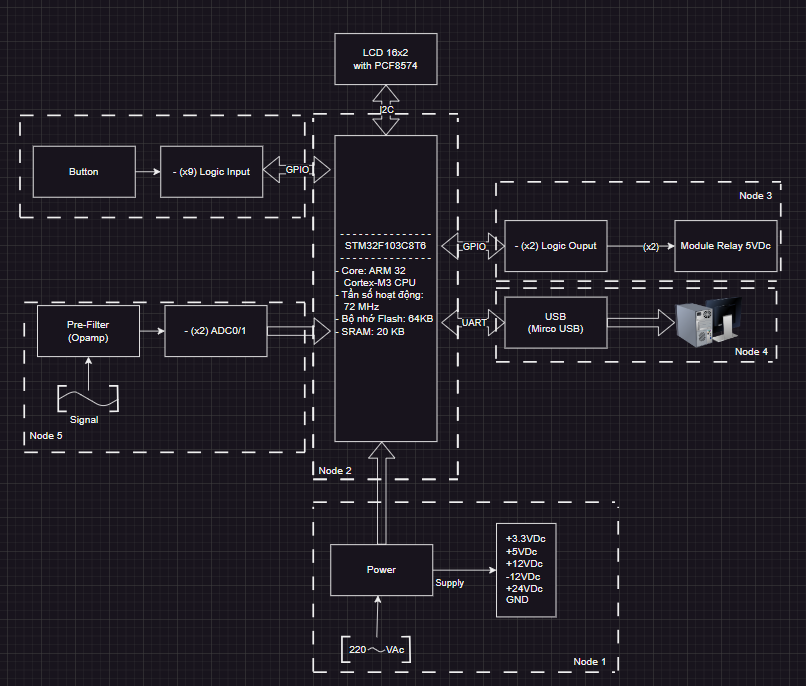
\includegraphics[width=\linewidth]{picture/Block Diagram.png}
	\begin{figure}[H]
		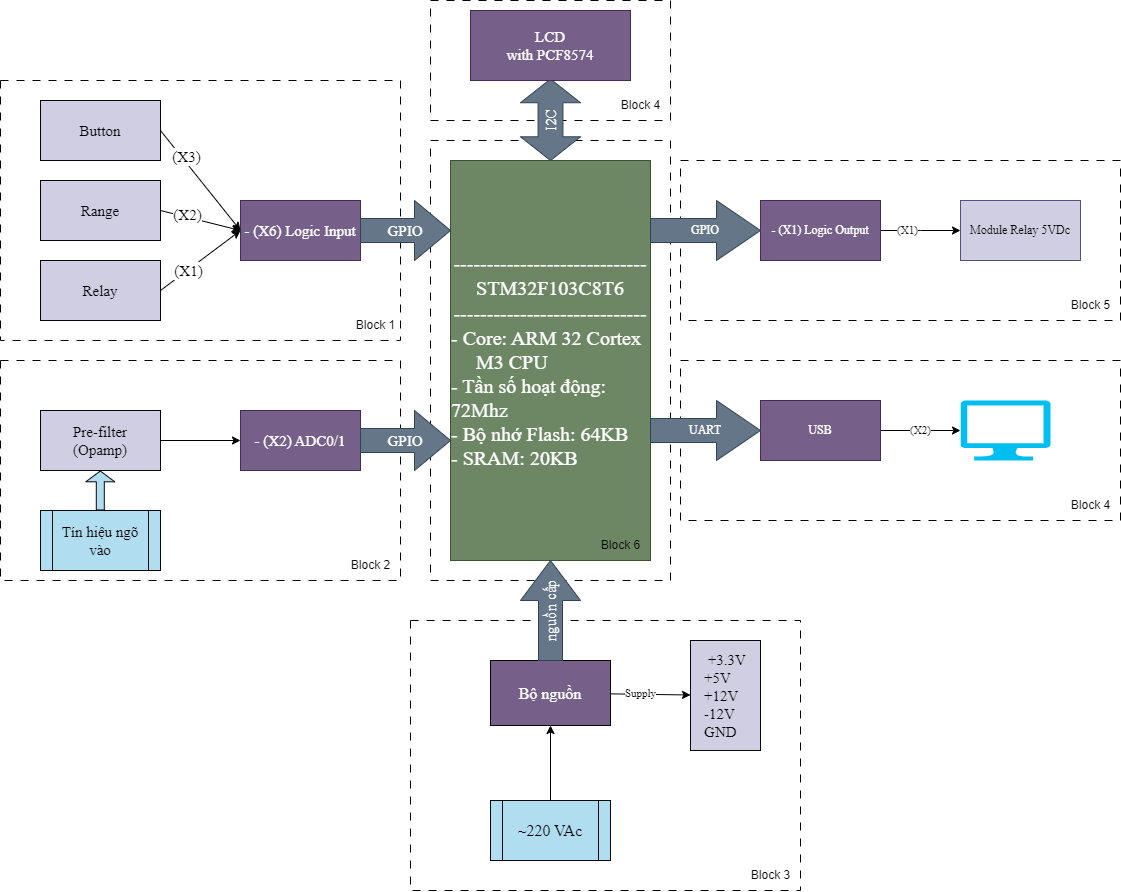
\includegraphics[width=\linewidth]{picture/system_block.png}
		\caption{System Block Diagram}
		\label{t_system block diagram}
	\end{figure}
	
	Khối được chia làm 6 phần chính:
	
	\begin{itemize}[label=-]
		\item Block 1: Có chức năng nhận dữ liệu từ nút nhấn, tín hiệu cho biết sử dụng ở thang đo nào, và tín hiệu khi có xuất hiện tín hiệu bảo vệ từ relay trả về.
		\item Block 2: Có chức năng nhận tín hiệu từ que đo vào khối xử lý thông qua chế độ đo sử dụng ADC.
		\item Block 3: Có chức năng cung cấp nguồn cho hệ thống.
		\item Block 4: Có chức năng hiển thị các giá trị của hệ thống ở chế độ AC hay DC trên LCD hoặc trên máy tính.
		\item Block 5: Có chức năng thực hiện điều khiển Relay để có thể chuyển chế độ đo giữa AC và DC.
		\item Block 6: Có chức năng xử lý chính các thao tác, các chương trình xử lý của hệ thống.
	\end{itemize}
	\item Power Block Diagram
	
	\begin{figure}[H]
		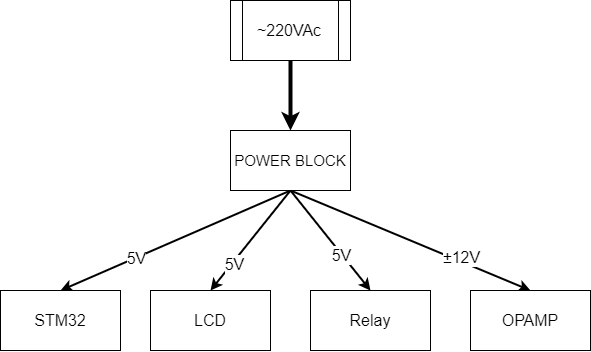
\includegraphics[width=\linewidth]{picture/power supply.png}
		\caption{Power Block Diagram}
		\label{t_power block diagram}
	\end{figure}
	%					
	%					Sơ đồ được chia làm 5 phần chính:
	%						\begin{itemize}[label=-]
		%							\item Khối nguồn
		%							\item Khối điều khiển
		%							\item Khối hiển thị và nút nhấn
		%							\item Khối giao tiếp với máy tính
		%							\item Khối tiền xử lý tín hiệu đầu vào
		%						\end{itemize}
	%					Đối với khối nguồn (Node 1): Sẽ sử dụng mạch nguồn được thiết sẵn.
	%					
	%					Đối với khối điều khiển (Node 2): Đóng vai trò là khối xử lý trung tâm xử lý tất cả các yêu cầu của hệ thống.
	%					
	%					Đôi 
\end{enumerate}
\section{Hardware specification}
\begin{itemize}[label = -]
	\item \textbf{DEVKIT STM32F103C8T6 Blue Bill}
	\begin{itemize}[label=+]
		\item \textbf{MCU: }STM32F103C8T6
		\item \textbf{Core: } ARM 32 Cortex-M3 CPU
		\item \textbf{Tần số hoạt động: } 72 MHz
		\item \textbf{Bộ nhớ Flash: } 64 KB
		\item \textbf{SRAM: } 20 KB
		\item \textbf{Điện áp I/O: } 2.0 $\sim$ 3.6 VDC
		\item \textbf{Thạch anh: } 16 MHz
		\item \textbf{Cổng MiniUSB: } Dùng để cấp nguồn và giao tiếp với các thiết bị ngoại vi.
		\item \textbf{Kích thước: } 5.3 x 2.2 cm
		\item \textbf{Sơ đồ nguyên lý (schematic) của DEVKIT STM32F103C8T6 Blue Bill}\\
		\begin{figure}[H]
			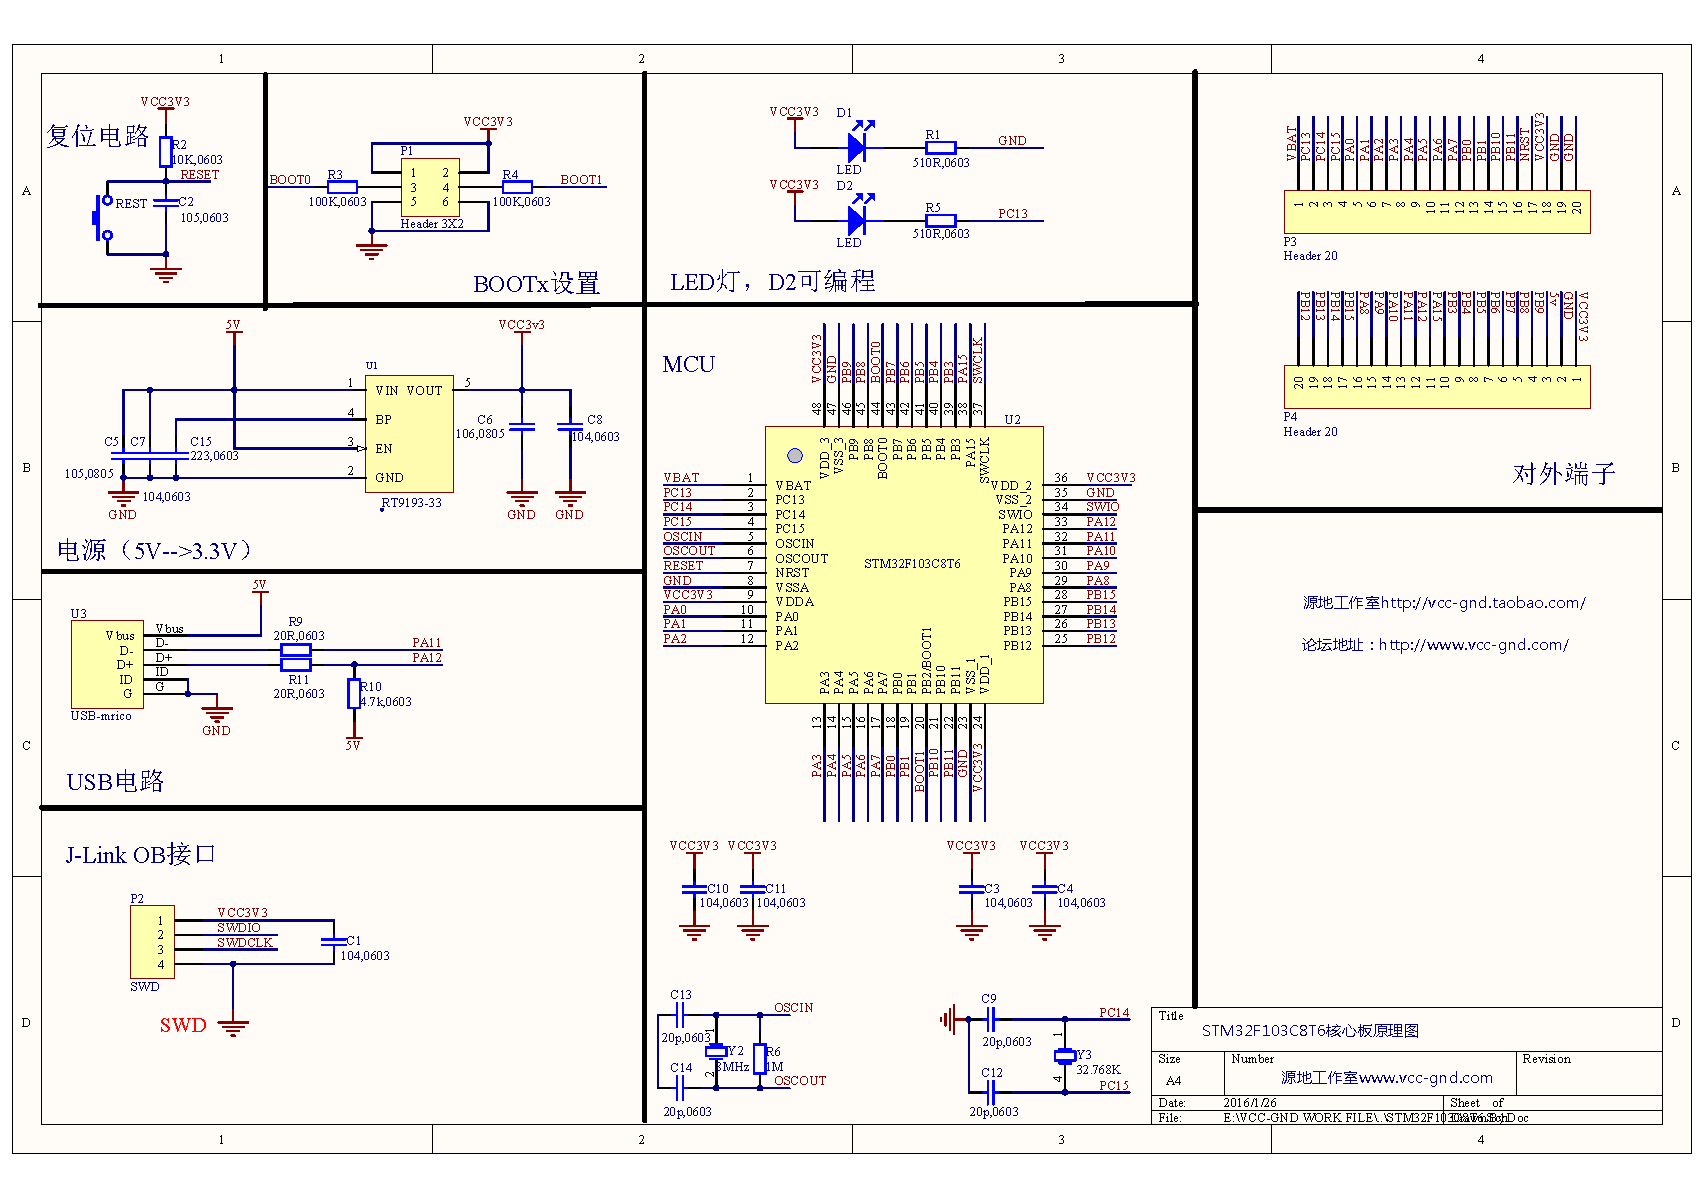
\includegraphics[ width = \linewidth]{original-schematic-STM32F103C8T6-Blue_Pill.pdf}
			\caption{Sơ đồ nguyên lý của Devkit STM32F103C8T6 Blue Bill}
			\label{t_schematic stm32 blue bill}
		\end{figure}
		\item \textbf{Sơ đồ chân Pin/ Pout:}\\
		\begin{figure}[H]
			\includegraphics[width=\linewidth]{picture/The-Generic-STM32F103-Pinout-Diagram.pdf}
			\caption{Sơ đồ chân của Devkit STM32F103C8T6 Blue Bill}
			\label{t_pin/pout stm32 blue bill}
		\end{figure}
	\end{itemize}
\end{itemize}
%	\item LCD 16x2 with PCF8547
%	\begin{itemize}[label=+]
%		\item Purpsse: Hiển thị các thông tin về các Mode hoạt động của hệ thống, hiển thị các giá trị của tín hiệu đầu vào như: Điện áp, Tần số, Điện áp hiệu dụng.
%		\item Requirement:
%		
%		\begin{tabularx}{\linewidth}{|p{0.2\linewidth}|p{0.2\linewidth}|p{0.2\linewidth}|p{0.3\linewidth}|}
%			\hline
%			Hardware component & Interface & Component Part Number & Note \\
%			\hline
%			LCD 16x2 with PCF8547 & I2C, 5V supply &  & \href{https://www.thegioiic.com/lcd-1602-nen-xanh-duong-chu-trang-5v-kem-i2c-driver}{LCD 1602 Nền Xanh Dương Chữ Trắng 5V Kèm I2C Driver} \\
%			\hline
%		\end{tabularx}
%	\end{itemize}
%	\item Module Relay 5VDc
%	\begin{itemize}[label=+]
%		\item Purpsse: Sử dụng để điều khiển trạng thái Mode của hệ thống.
%		\item Requirement:
%		
%		\begin{tabularx}{\linewidth}{|p{0.2\linewidth}|p{0.2\linewidth}|p{0.2\linewidth}|p{0.3\linewidth}|}
%			\hline
%			Hardware component & Interface & Component Part Number & Note \\
%			\hline
%			Module Relay 5VDc & 5V supply &  & \href{https://cafelinhkien.com/san-pham/module-relay-2-kenh-5vdc/}{Module Relay 2 Kênh 5VDC} \\
%			\hline
%		\end{tabularx}
%	\end{itemize}
%	\item OPAMP TL082
%	\begin{itemize}[label=+]
%		\item Purpsse:Sử dụng trong khối tiền xử lý tín hiệu để kiểm soát chất lượng tín hiệu đầu vào khối xử lý giúp cho kết quả xử lý được đảm bảo về mặt chính xác hơn.
%		\item Requirement:
%		
%		\begin{tabularx}{\linewidth}{|p{0.2\linewidth}|p{0.2\linewidth}|p{0.2\linewidth}|p{0.3\linewidth}|}
%			\hline
%			Hardware component & Interface & Component Part Number & Note \\
%			\hline
%			TL082CP & \href{https://www.ti.com/lit/ds/symlink/tl082.pdf?ts=1690260841562}{Datasheet} & Texas Instruments & \href{https://www.thegioiic.com/tl082cp-ic-j-fet-amplifier-2-circuit-4-mhz-8-dip}{TL082CP IC J-FET Amplifier 2 Circuit 4 MHz, 8-DIP} \\
%			\hline
%		\end{tabularx}
%	\end{itemize}

	\section{Software Specification}
	\begin{itemize}[label=-]
		\item Chức năng chính của hệ thống:\\
		\begin{figure}[H]
			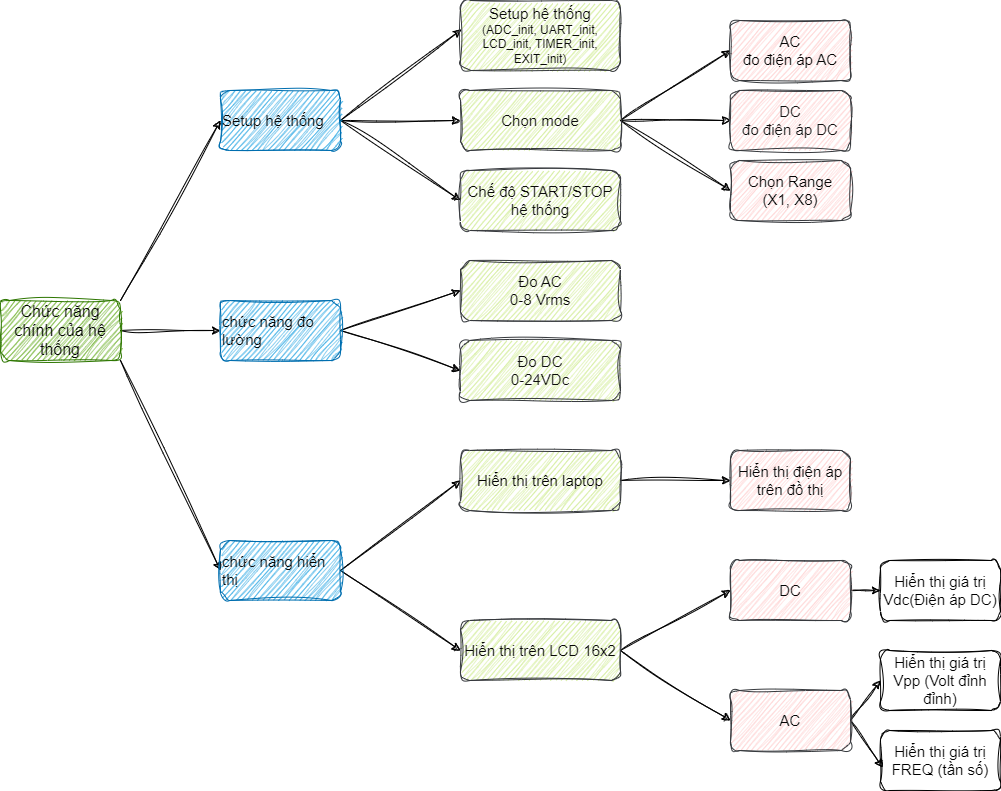
\includegraphics[width=\linewidth]{picture/software_flowchart.png}
			\caption{Software Specification}
			\label{t_software specification}
		\end{figure}
	\end{itemize}
	
	\section{Test Specification}
	\begin{itemize}[label=-]
		\item Device:
		\begin{itemize}[label=+]
			\item Voltage meter
			\item Breadboard
		\end{itemize}
		\item Test Processing:
		\begin{itemize}[label=+]
			\item Xem các chức năng và thông số hiển thị trên LCD có đúng không.
			\item Các thông số được gửi lên máy tính có đáp ứng được yêu cầu của hệ thông hay không.
			\item Thực hiện kiểm chứng cách chức năng của hệ thống với các lựa chọn Mode khác nhau.
		\end{itemize}
	\end{itemize}

	
	%					\item \textbf{Hệ điều hành và phát triển}
	%					\begin{itemize}[label=-]
		%						\item \textbf{FreeRTOS: }Đây là hệ điều hành thời gian thực phổ biến và miễn phí được sử dụng rộng rãi với STM32F103C8T6. FreeRTOS cung cấp các tính năng như quản lý đa nhiệm, đồng bộ hóa và giao tiếp giữa các tác vụ, thích hợp cho các ứng dụng cần đáp ứng nhanh và đáng tin cậy.
		%						\item \textbf{CMSIS-RTOS: }Phần mềm cung cấp một API thống nhất cho việc phát triển ứng dụng với ARM Cortex-M, hỗ trợ RTOS và không RTOS. CMSIS-RTOS API được hỗ trợ bởi RTX (Keil RTX) và FreeRTOS.
		%						\item \textbf{ChibiOS/RT: }Đây là một hệ điều hành thời gian thực nhẹ và hiệu quả, cung cấp quản lý đa nhiệm và đồng bộ hóa với một bộ thư viện phong phú hỗ trợ các ngoại vi của STM32.
		%						\item \textbf{Zephyr: }Một RTOS mã nguồn mở được phát triển cho IoT và các thiết bị nhúng. Zephyr có kiến trúc module linh hoạt, bảo mật mạnh mẽ và hiệu năng cao.
		%						\item \textbf{STM32CubeIDE: }Đây là một IDE dựa trên Eclipse tích hợp các công cụ cấu hình phần cứng và lập trình cho STM32. STM32CubeIDE hỗ trợ lập trình, nạp chương trình, và gỡ lỗi (debugging) trên STM32F103C8T6.
		%						\item \textbf{Arduino }IDE: STM32F103C8T6 cũng có thể lập trình bằng Arduino IDE nhờ hỗ trợ từ thư viện Arduino Core cho STM32. Điều này giúp đơn giản hóa việc lập trình cho những người mới bắt đầu.
		%					\end{itemize}
	%					\item \textbf{Sơ đồ nguyên lý (schematic) của DEVKIT STM32F103C8T6 Blue Bill}
	%					
	%					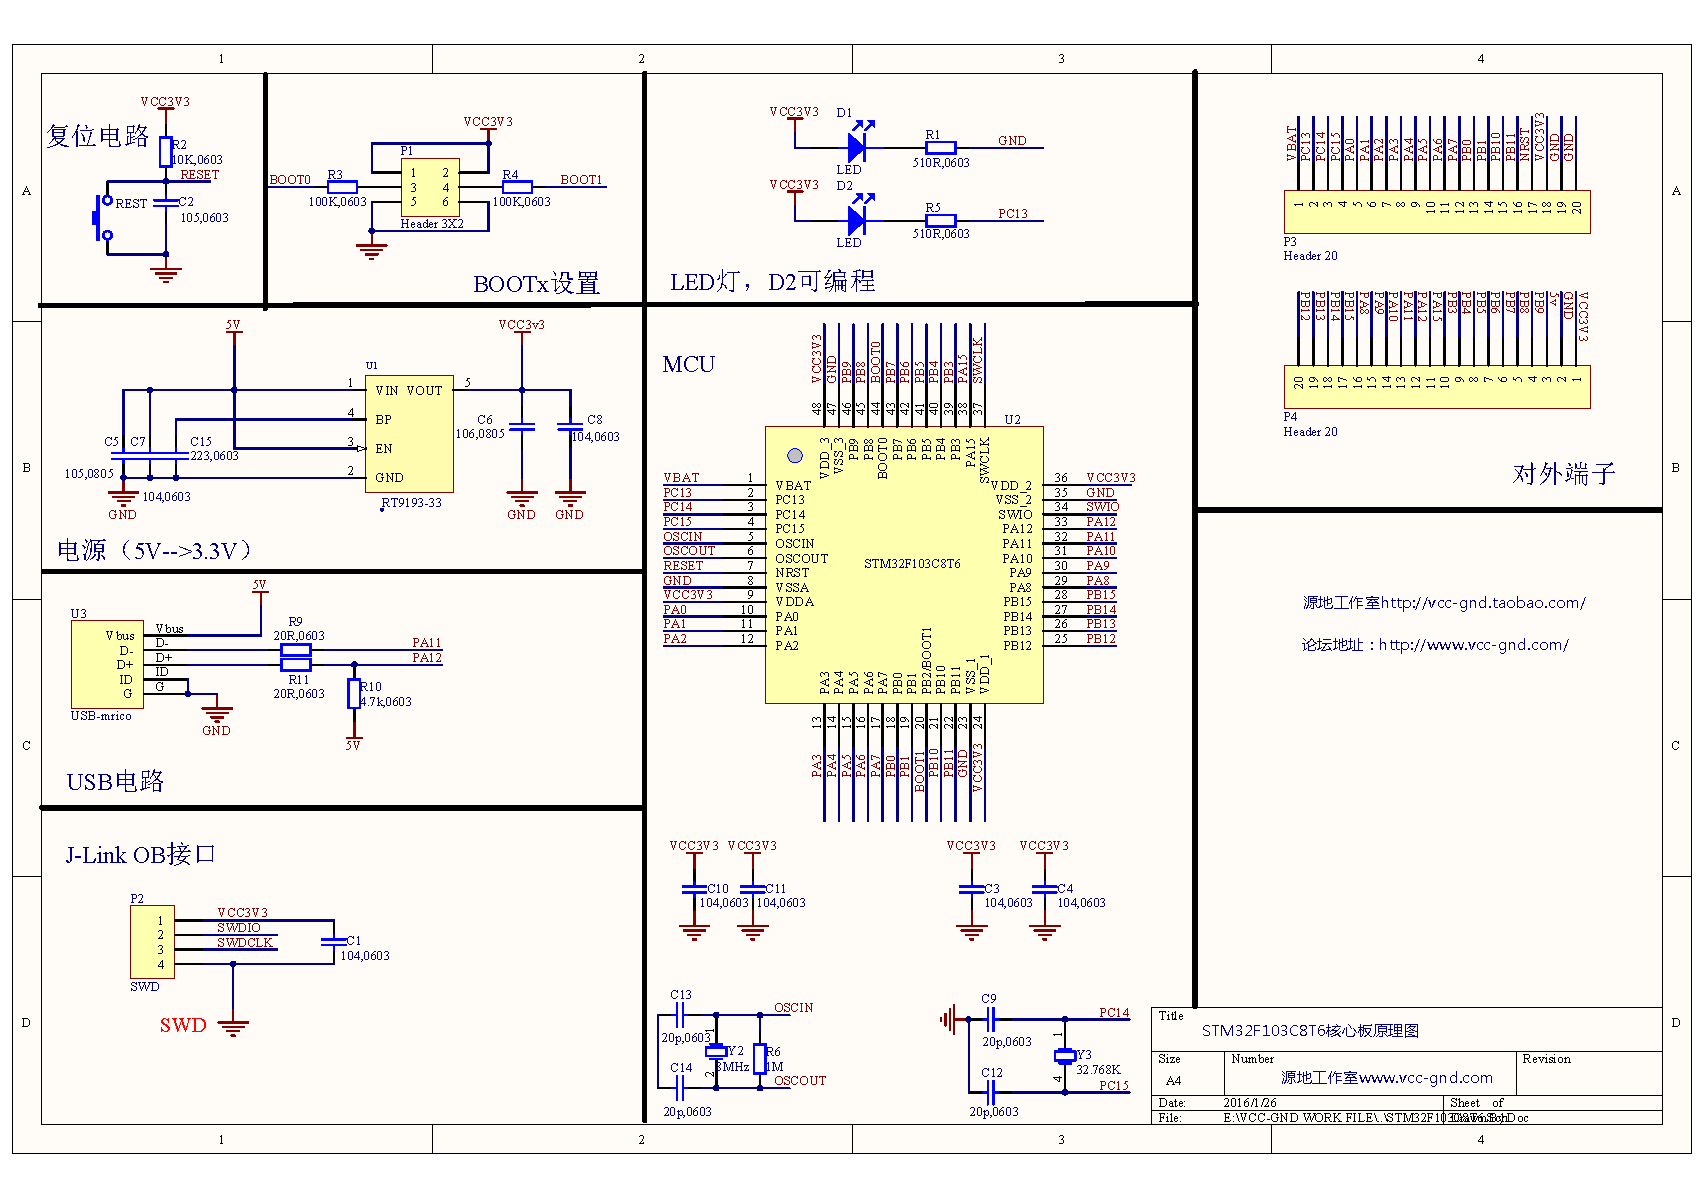
\includegraphics[width = \linewidth]{original-schematic-STM32F103C8T6-Blue_Pill.pdf}
	%					
	%					\item \textbf{Sơ đồ chân Pin/ Pout:}
	%					
	%					\includegraphics[width=\linewidth]{picture/The-Generic-STM32F103-Pinout-Diagram.pdf}
	%				\end{itemize}